\newcommand*{\tou}[1]{\textcolor{Brown}{#1}}

\section{Versuchsaufbau und -durchführung}
	In allen Experimenten wird das Spülmittel "Limonen Spülmittel" von Frosch verwendet. Der Handelsname entspricht "FROSCH LIMONEN SPÜLMITTEL EF 750 ML D".
	\subsection{Aufstieg von Luftblasen}
		\begin{tabularx}{\textwidth}{l X}
			\tou{Versuchsziel} & Bestimmung der Viskosität von Spülmittel durch Beobachtung des Blasenaufstiegs in Abhängigkeit von der Temperatur \\
			\tou{Messmethode} & Kamera und das Software \texttt{osp-tracker}\footnote{\url{physlets.org/tracker/}}
		\end{tabularx}
		\begin{enumerate}
			\item \textbf{Bestimmung der Dichte}

				Zur Bestimmung der Dichte des Spülmittels wird eine halbgefüllte Spülmittelfläsche ins Wasser schwimmen gelassen. So funktioniert die Fläsche als einen Aräometer. Die Höhe des Wasserpegels wird dann auf das Fläsche mit einem Marker markiert und die Höheunterschied mittels \texttt{osp-tracker} bestimmt.
				\vspace{\baselineskip}
				\begin{multicols}{2}
					\begin{figure}[H]
						\centering
						\includegraphics[width=0.3\textwidth]{tv1-dichte1.jpg}
						\caption{\centering Aräometer Aufbau}
					\end{figure}
					\begin{figure}[H]
						\centering
						\includegraphics[width=0.3\textwidth]{tv1-dichte2.jpg}
						\caption{\centering Bestimmung der Höhe des Wasserpegels}
					\end{figure}
				\end{multicols}
				Sodass das Volumen des verdrängtes Wassers genauer bekannt ist, ist der $\SI{10}{\liter}$ Eimer in einer große Schüssel gelagert. Das verdrängte Wasser ist dann in dieser Schüssel aufgefangen und deren Volumen mit einem Messbecher bestimmt. 

				Die bestimmte Dichte wird dann mit den vom Hersteller angegebenen Werten und den aus einen Aräometer ermittelten Werten verglichen.
			\item \textbf{Aufstieg von Luftblasen}

				Das Spülmittel ist dann $1$ Stunde lang im Raum gelagert, damit es die Temperatur der Umgebung angenommen hat. Die gemessene Temperatur war $\SI{29(1)}{\celsius}$. 

				Anstelle der vorgeschriebenen Schüttelmethode sind Luftblasen durch Pusten in einem Strohhalm produziert. Dadurch ist die Blasenproduktion besser kontrolliert und man muss nicht darauf warten, dass die kleine Blasen verschwinden, wenn zu viele kleine Blasen durch das Schütteln entstehen, was den Aufstieg von größeren Blasen verhindert. Die Größe der Luftblasen wurden aber dadurch etwa größer sein.

				Der Aufstieg der Luftblasen wurden dann mit einem Handycamera bei $60$ Bilder pro Sekunde aufgenommen. Das Handy war ein SAMSUNG S10e mit der Auflösung von $1080$x$1920$ Pixels (d.h. vertikale Ausrichtung) und einem Zoomfaktor von $1.0$x. 
				\begin{figure}[H]
					\centering
					\captionsetup{width=0.8\linewidth, justification=centering}
					\includegraphics[width=0.75\linewidth]{tv1-setup.jpg}
					\caption{Experiment Aufbau\\Das Handy wird während des Experiments mit einem Klebeband aufrechts gehalten.}
					\vspace{-1em}
					\label{fig:exp-setup}
				\end{figure}
				Die Auswertung erfolgt dann in \texttt{osp-tracker}. Dabei sind die Durchmesser und Positionen gemessen.
				\begin{figure}[H]
					\centering
					\captionsetup{width=0.8\linewidth, justification=centering}
					\includegraphics[width=0.8\linewidth]{tv1-tracker.png}
					\caption{Auswertung in \texttt{osp-tracker}}
				\end{figure}
				Der Aufstieg von $10$ Luftblasen wurden aufgenommen. 
				\begin{figure}[H]
					\centering
					\captionsetup{width=0.8\linewidth, justification=centering}
					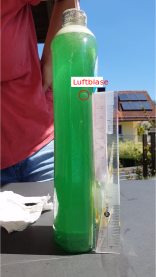
\includegraphics[width=0.5\linewidth]{tv1-aufstieg.eps}
					\caption{Ein solcher Aufstieg}
				\end{figure}
				\begin{multicols}{2}
					Das Spülmittel wurde dann im Gefrierschrank für $2$ Stunden gelagert und dann grob geschüttelt, sodass die Temperatur des Spülmittels überall gleich war. Die gemessene Temperaturen waren:
					\begin{center}
						\begin{tabular}{ll}
							\toprule
							Anfangstemperatur $\theta_i$ & \SI{4(1)}{\celsius} \\
							Endtemperatur $\theta_{\!f}$ & \SI{12(1)}{\celsius} \\
							\bottomrule
						\end{tabular}
					\end{center}
					Das Experiment wurden dann mit $10$ Luftblasen im kalten Spülmittel wiederholt. Es ist beobachtet, dass die Luftblase im kalten Spülmittel wie einen umgekehrten Tropfen aussah.
					\columnbreak
					\begin{figure}[H]
						\centering
						\captionsetup{width=0.45\linewidth, justification=centering}
						\includegraphics[width=0.4\linewidth]{tv1-cold.png}
						\caption{Luftblasen im kalten Spülmittel}
					\end{figure}
				\end{multicols}
				Wegen der unkugelförmigen Form der Luftblasen im kalten Spülmittel, ist ein Kreis am oberen Teil der Blase erst angepasst, bevor die Messungen des Durchmesser durchgeführt sind. Da die Luftblasen in der Bewegungsrichtung immer noch kugelförmig ist, ist das eine gute Annäherung dafür.
				\begin{figure}[H]
					\centering
					\captionsetup{width=0.7\linewidth, justification=centering}
					\includegraphics[width=0.6\linewidth]{tv1-cold-dia.png}
					\caption{Messungen des Durchmessers im kalten Spülmittel in \texttt{osp-tracker}}
					\vspace{-1em}
				\end{figure}
				Um möglichst wenig Verformung in der Aufnahmen zu haben, ist die Spülmittelflasche von der Seite gefilmt, wo die Wand flacher ist. Die Luftblasen sind auch möglichst nah an der Wand erzeugt. Dies gilt für den ganzen Teilversuch. 
		\end{enumerate} 
	\newpage
	\subsection{Kugelfallviskosimeter}

		\begin{tabularx}{\textwidth}{l X}
			\tou{Versuchsziel} & Bestimmung der Viskosität von Spülmittel bei Raumtemperatur mit einem improvisierten Kugelfallviskosimeter \\
			\tou{Messmethode} & Kamera und das Software \texttt{osp-tracker}
		\end{tabularx}

		Eine Wasserfläsche wurde mit Spülmittel bei $T=\SI{33(1)}{\celsius}$ gefüllt und als Kugelfallviskosimeter verwendet. Stahlkugeln aus einem magenetisches Konstruktionsspielzeug sind dann mit einer Schieblehre gemessen und dann mit Spiritus ($70\%$ v/v Ethanol) gereinigt. 

		Die Stahlkugeln haben folgenden Eigenschaften:
		\begin{center}
			\begin{tabular}{ll}
				\toprule
				Masse $m$ & \SI{8.5(2)}{\gram} \\
				Durchmesser $d$ & \SI{12.7(1)}{\milli\meter} \\
				\bottomrule
			\end{tabular}
		\end{center}
		wobei die Masse $m$ aus einer Messung aus $15m = \SI{127(3)}{\gram}$ hergeleitet ist. 

		Die Spülmittelflasche in Abbildung \ref{fig:exp-setup} wurde mit dem Kugelfallviskosimeter ersetzt und die Stahlkugel ins Spülmittel fallen gelassen. Dazu sind die Kugeln nach der Reinigung nur mit Pinzette behandelt. Der Fallverlauf wurde dann mit dem gleichen Handy und der gleichen Einstellungen wie in dem vorherigen Versuch aufgenommen. 

		Die Messung der Zeit und Position erfolgt danach im \texttt{osp-tracker}.
		\begin{figure}[H]
			\centering
			\captionsetup{width=0.8\linewidth, justification=centering}
			\includegraphics[width=0.9\linewidth]{tv2-tracker.png}
			\caption{Auswertung in \texttt{osp-tracker}}
		\end{figure}
		Diese Messungen sind für insgesamt $9$ Stahlkugeln wiederholt.